%%%%%%%%%%%%%%%%%%%%%%%%%%%%%%%%%%%%%%%%%%%%%%%%%%%%%%%%%%%%%%%%%%%%%%%%

%%% Empty Two Column LaTeX Template (Based on AAMAS-2023 (based on sample-sigconf.tex))

\documentclass[sigconf,nonacm]{acmart}

%%% Load required packages here (note that many are included already).

\usepackage{balance} % for balancing columns on the final page
\usepackage{float}
\usepackage{stfloats}

\newcommand{\argmax}{\mathop{\mathrm{argmax}}}

\title[RL Bachelor]{
    Assignment 1b: Dynamic Programming
}

\author{Peter Huijsen (s4516303) \& Ahmed Al Kurwi (s4476581)}
\affiliation{
    Group Number: 43
    \country{} \institution{} \city{} % Just included empty to avoid some warnings
}

%%%%%%%%%%%%%%%%%%%%%%%%%%%%%%%%%%%%%%%%%%%%%%%%%%%%%%%%%%%%%%%%%%%%%%%%

% Keep this part as is
\begin{document}
\pagestyle{fancy} 
\lhead{}
\rhead{Introduction to Reinforcement Learning, Leiden University, 2026}
\maketitle 

%%%%%%%%%%%%%%%%%%%%%%%%%%%%%%%%%%%%%%%%%%%%%%%%%%%%%%%%%%%%%%%%%%%%%%%%

\section{Introduction}
In reinforcement learning (RL), an agent learns to make decisions in an environment by taking actions. From these actions, the agent receives some reward or penalty from the environment.

This paper explores a specific type of RL agent that uses a Markov-Decision Process (MDP) to plan and solve a fully observable environment. This entails that the agent can only learn in a fully observable environment, and as such, it does not use any exploration to improve its decisions. It does this through calculating a policy from the current expected reward of each action in each state, and taking the action that maximizes this reward. In this manner, its policy improves every iteration until it converges to the optimal policy.

This paper shows that this RL agent is quite effective in small, limited, fully observable environments when implemented using dynamic programming (DP). With this method, the state-space that needs to be explored by memorizing the results of subproblems is significantly reduced. However, the limitations of this agent, both computationally, i.e., the curse of dimensionality, and in general, should also be noted.

\begin{figure}[H]
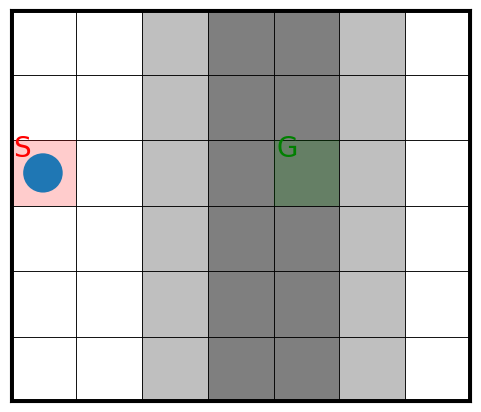
\includegraphics[width=0.65\linewidth]{figures/environment.png}
\caption{
    The environment used throughout the experiment, where the agent is able to move up, down, left, or right. It receives a reward of $-1$ for each move, and a reward of $35$ when reaching the green cell. The shaded cells push the agent upwards by one cell for columns three and six, or two cells for columns four and five.
}
\label{fig:world}
\end{figure}

A specific grid environment is used throughout this paper to explore the behavior of this agent. In this environment, the agent, shown as the blue circle, starts in the red cell. From each cell, the agent is able to move up, down, left, or right. However, the cells shaded in columns three and six push the agent up one cell, while the cells shaded in columns four and five push the agent up two cells. If the agent reaches the green cell, it receives a reward of $+35$, while each step the agent takes gives it a reward of $-1$.

\section{Methods}
The goal of the MDP agent is to find an optimal policy $\pi^*$. This is based upon a number of building blocks given by the environment. First, a state and action space are needed, $\mathcal{S}$ and $\mathcal{A}$ respectively. Then, the transition function $p(s'|s,a)$ defines the probability distributions of the resulting states for each state-action combination. Next, a reward function $r(s,a,s')$ is needed to define the given reward for the combination of state-action and resulting states. Finally, a discount factor $\gamma\in[0,1]$ and initial state probability distribution $p_0(s)$ are needed. The expected reward for a given policy is described by the $Q_\pi$ matrix, which contains this expectation for each state-action combination.

The agent learns through policy iteration, which consists of two phases:
\begin{enumerate}
    \item \textbf{Policy evaluation}: continuously update the current expected rewards for each state-action combination by the state-action value Bellman equation shown in Equation~\ref{eq:bellman} until convergence, that is, the difference between the last and current update is less than some small threshold. Here, the discount factor is used to weigh more recent rewards more than future rewards, and as such, encourages the agent to find an efficient solution. If this value were set to one, then each subsequent reward used in its calculations would be weighed equally to earlier gotten rewards.
    \begin{equation}
        Q_\pi(s,a)\leftarrow\mathbb{E}_{s'\sim p}\left[r+\gamma\cdot\mathbb{E}_{a'\sim\pi}\left[Q_\pi(s',a')\right]\right]
        \label{eq:bellman}
    \end{equation}
    \item \textbf{Policy improvement}: update the current policy by the new expected rewards, as shown in Equation~\ref{eq:policy}:
    \begin{equation}
        \pi(s)\leftarrow \argmax_{a}\space Q_\pi(s,a)
        \label{eq:policy}
    \end{equation}
\end{enumerate}
Now, policy iteration continues until the resulting policy converges to an unchanging policy. In general, any process that improves and evaluates a policy is a Generalized Policy Iteration (GPI) algorithm, such as policy iteration itself. Therefore, there are other options available, such as value iteration (VI).

Here, the discount factor in the Bellman equation is used to incentivize short-term rewards, i.e., prefers more efficient paths for $\gamma<1$. In addition, the cumulative reward stays bounded, ensuring the Bellman equation converges. 

When implementing such a GPI algorithm, DP is a good tool to use since the recursive relationship of $Q(s,a)$ can be split up into separate subproblems to solve and memoize. As such, the amount of computation needed can be greatly reduced. The VI algorithm takes advantage of this by using the Bellman optimality equation, shown in Equation~\ref{eq:bellman_optimality}. The iterations in the policy evaluation step can then be condensed into one single iteration over the entire state-action space.
\begin{equation}
     Q_\pi(s,a)\leftarrow\mathbb{E}_{s'\sim p}\left[r+\gamma\cdot\max_{a'}\space Q_\pi(s',a')\right]
    \label{eq:bellman_optimality}
\end{equation}
Then, the policy can be computed again, as shown in Equation~\ref{eq:policy}. This is significantly more efficient than computing many iterations within policy evaluation before converging.

However, a disadvantage of using DP in this manner is the curse of dimensionality: when an environment gets larger and more complex, the resulting $Q$ values that need to be stored explode exponentially. As such, it rapidly becomes computationally impractical to use this method to compute the optimal policy.

\begin{figure*}[t!]
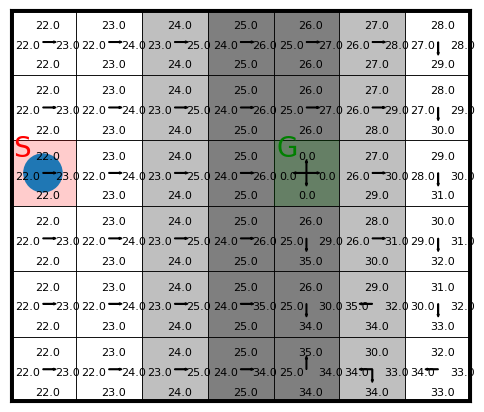
\includegraphics[width=0.32\linewidth]{figures/mdp.png}
\hfill
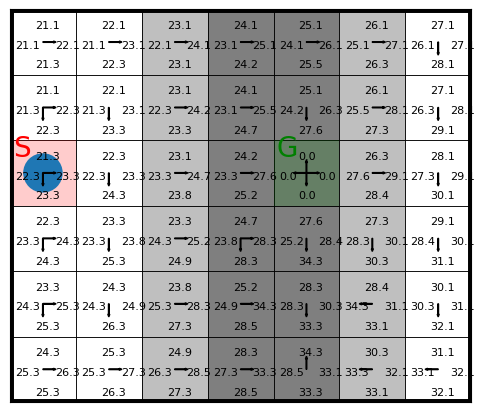
\includegraphics[width=0.32\linewidth]{figures/mdp_stochastic.png}
\hfill

\includegraphics[width=0.32\linewidth]{1b/figures/mdp_non_discount.png}
\caption{
   First, an MDP VI solution with $\gamma=1.0$, where in each cell the arrow points in the direction in which it is optimal to move to from that state. If there are two arrows, both actions have an equal expected reward and are thus both optimal. It is optimal for the agent to navigate around the edge of the environment, since otherwise it would get pushed from the goal by the wind. Next, a solution is shown with a stochastic environment where $p_{wind}=0.75$. As such, it is now more advantageous to directly move towards the goal. Finally, a solution is shown with $\gamma=1.0$, and where the agent does not receive a penalty for taking an action. Since the agent does not get punished for taking an action, and the reward is not discounted over time, it does not matter what action the agent takes, since it will inevitably reach the reward eventually.
}
\label{fig:mdps}
\end{figure*}

\section{Results}
To evaluate the VI agent, three distinct environment configurations were examined, as shown in Figure \ref{fig:mdps}. 

In the standard environment, which contains a step penalty, the agent learns to navigate through the wind columns and use them to reach its goal, allowing itself to be pushed upwards towards the top edge. When having reached the right side, the agent moves down again and uses the wind to reach the goal. In this manner, the agent reaches the goal with the least amount of steps, and as such with the most reward remaining since its reward per step is $-1$, i.e., a penalty.

Next, in the stochastic environment with $p_{wind}=0.75$, the optimal policy is shifted to a more direct trajectory. Since the wind no longer blows the agent upwards on every step, and only has a $75\%$ chance of blowing the agent upwards, the expected reward of moving through the wind columns is much higher than in the original scenario. Thus, the policy of the agents changes to reflect this new optimal strategy. The agent can deal with this stochasticity since the Bellman equation computes the expectation of all possible resulting states. In the standard environment, there was simply only one possible resulting state from the state transition function.

Finally, the step penalty is removed, still using a discount factor of $\gamma=1.0$. As such, the agent does not care about efficiency. So, any path of any length that reaches the goal gives a reward of $+35$, which results in uniform $Q$-values across all states and a random policy where it wanders around aimlessly until it happens to reach the goal. Lowering the discount factor to $\gamma=0.95$ restores optimal behavior since future rewards now lose their value over time. Thus, to achieve the optimal reward in the Bellman equation, the number of steps again matters, even though there is no penalty. Each step reduces the reward by five percent.

\section{Discussion \& Conclusion}

This paper shows that an agent can solve fully observable, small RL problems using MDPs and DP. Using DP to optimize PI and condense its two phases into one for VI greatly improves general performance. However, the $Q$ values that need to be stored increase rapidly when adding more states or actions, and as such, this curse of dimensionality limits the applications of this direct method.

The Bellman equations shown are used by these GPIs to compute the optimal policy. In these equations, the discount factor $\gamma$ encourages efficiency and ensures convergence. 

This paper has shown how MDPs work and how they can be implemented with DP, however only state-action value methods were shown in this paper, while state value methods are also widely used. Additionally, the environment used in this paper is relatively simple: it only includes one reward, and its stochasticity is quite limited. As such, a more complex environment could demonstrate the complexities of GPI more effectively. 

Future work could solve this by implementing a Neural network. Rather than storing a discrete $Q$-value for every possible state-action pair in a 2D array, the agent would use a deep neural network to approximate the values. This would allow the agent to generalize its learning and be able to perform in larger environments. Other future work could analyze how the agent for stochastic wind performs when there is a huge penalty if the agent gets pushed too far up to see if the agent would act differently and take fewer risks, or act the exact same.

\newpage

%%% The following command should be issued somewhere in the first column 
%%% of the final page of your paper.
\balance

%%%%%%%%%%%%%%%%%%%%%%%%%%%%%%%%%%%%%%%%%%%%%%%%%%%%%%%%%%%%%%%%%%%%%%%%

%%% The next two lines define, first, the bibliography style to be 
%%% applied, and, second, the bibliography file to be used.

\end{document}

%%%%%%%%%%%%%%%%%%%%%%%%%%%%%%%%%%%%%%%%%%%%%%%%%%%%%%%%%%%%%%%%%%%%%%%%

